\documentclass{cubeamer}

\title{Introdução a modelagem 3D}
\subtitle{Workshop de Arduino - \textbf{rascimatec}}
\author[Tiago Barretto Sant'Anna]{Tiago Barretto Sant'Anna.}
\date{\today} % or whatever the date you are presenting in is
\institute[SENAI CIMATEC]{SENAI CIMATEC - IEEE ROBOTICS AND AUTOMATION SOCIETY}
% \copyrightnotice{Published by the American Institute of Aeronautics and Astronautics, Inc., with permission}
\usepackage{ragged2e}
\begin{document}

\maketitle

\cutoc

\section{O que é o Onshape}

\begin{frame}{O que é modelagem 3D?}
    \begin{columns}

        \begin{column}{0.4\textwidth}
            \begin{itemize}
                \item Conceito base
                \item CAD (Desenho assistido por computador)
                \item Aplicações
            \end{itemize}
        \end{column}

        \begin{column}{0.6\textwidth}
            \begin{figure}
                \centering
                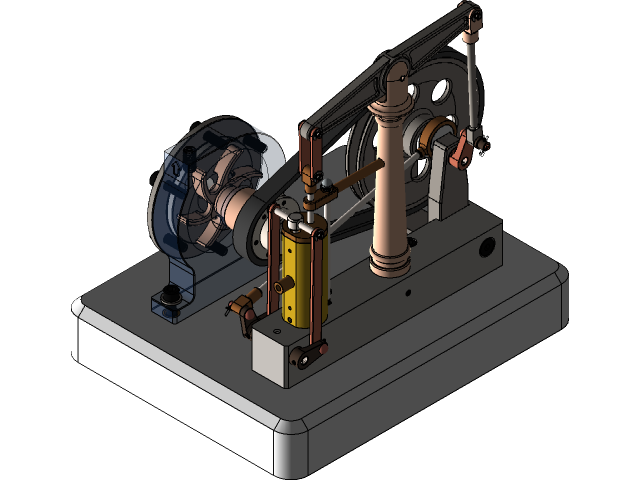
\includegraphics[height = 0.7\textheight]{img/bomba.png}
                \caption{\cite{Bomba:online}}
            \end{figure}
        \end{column}

    \end{columns}
\end{frame}

\begin{frame}{Porque usar o Onshape?}
    \begin{columns}

        \begin{column}{0.5\textwidth}
            \begin{itemize}
                \item Licença educacional
                \item Online
                \item Multi-plataforma
                \item Facil compartilhamento de arquivos
                \item Multipla edição
                \item Versionamento de arquivos
            \end{itemize}
        \end{column}

        \begin{column}{0.5\textwidth}
            \begin{figure}
                \centering
                
\includegraphics[height = 0.6\textheight]{img/onshape.png}
                \caption{\cite{Onshape:online}}
            \end{figure}
        \end{column}

    \end{columns}
\end{frame}

\section{Desenho técnico}

\begin{frame}{Para que desenho tecnico?}
    \begin{columns}
        \begin{column}{0.5\textwidth}
            \begin{itemize}
                \item Forma de representação
                \item Obter medidas
            \end{itemize}
        \end{column}

        \begin{column}{0.5\textwidth}
            \begin{figure}
                \centering
                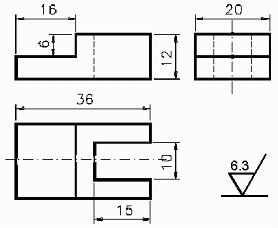
\includegraphics[height = 0.6\textheight]{img/desenho1.jpg}
                \caption{\cite{listade:online}}
            \end{figure}
        \end{column}
    \end{columns}
\end{frame}

\begin{frame}{Linhas}
    \begin{center}
        \begin{figure}
            \centering
            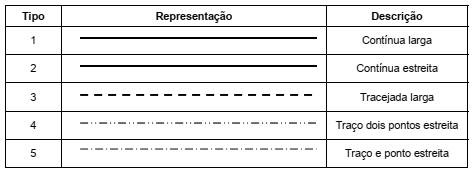
\includegraphics[height = 0.6\textheight]{img/desenho.png}
            \caption{\cite{linha:online}}
        \end{figure}
    \end{center}
\end{frame}

\begin{frame}{Vistas}
    \begin{center}
        \begin{figure}
            \centering
            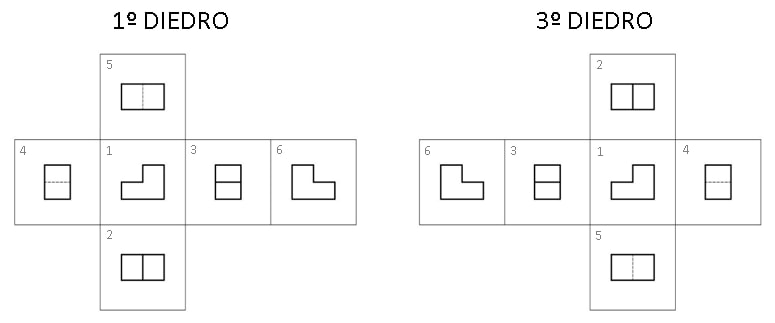
\includegraphics[height = 0.6\textheight]{img/desenho4.jpg}
            \caption{\cite{diedro:online}}
        \end{figure}
    \end{center}
\end{frame}

% /TODO TROCAR IMAGEM
\begin{frame}{Cotagem}
    \begin{center}
        \begin{figure}
            \centering
            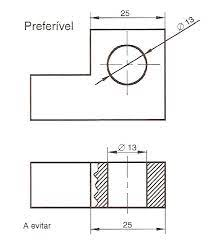
\includegraphics[height = 0.6\textheight]{img/desenho5.jpeg}
            \caption{\cite{cota:online}}
        \end{figure}
    \end{center}
\end{frame}

\begin{frame}{Exemplos}

    \begin{columns}
        \begin{column}{0.5\textwidth}
            \begin{figure}
                \centering
                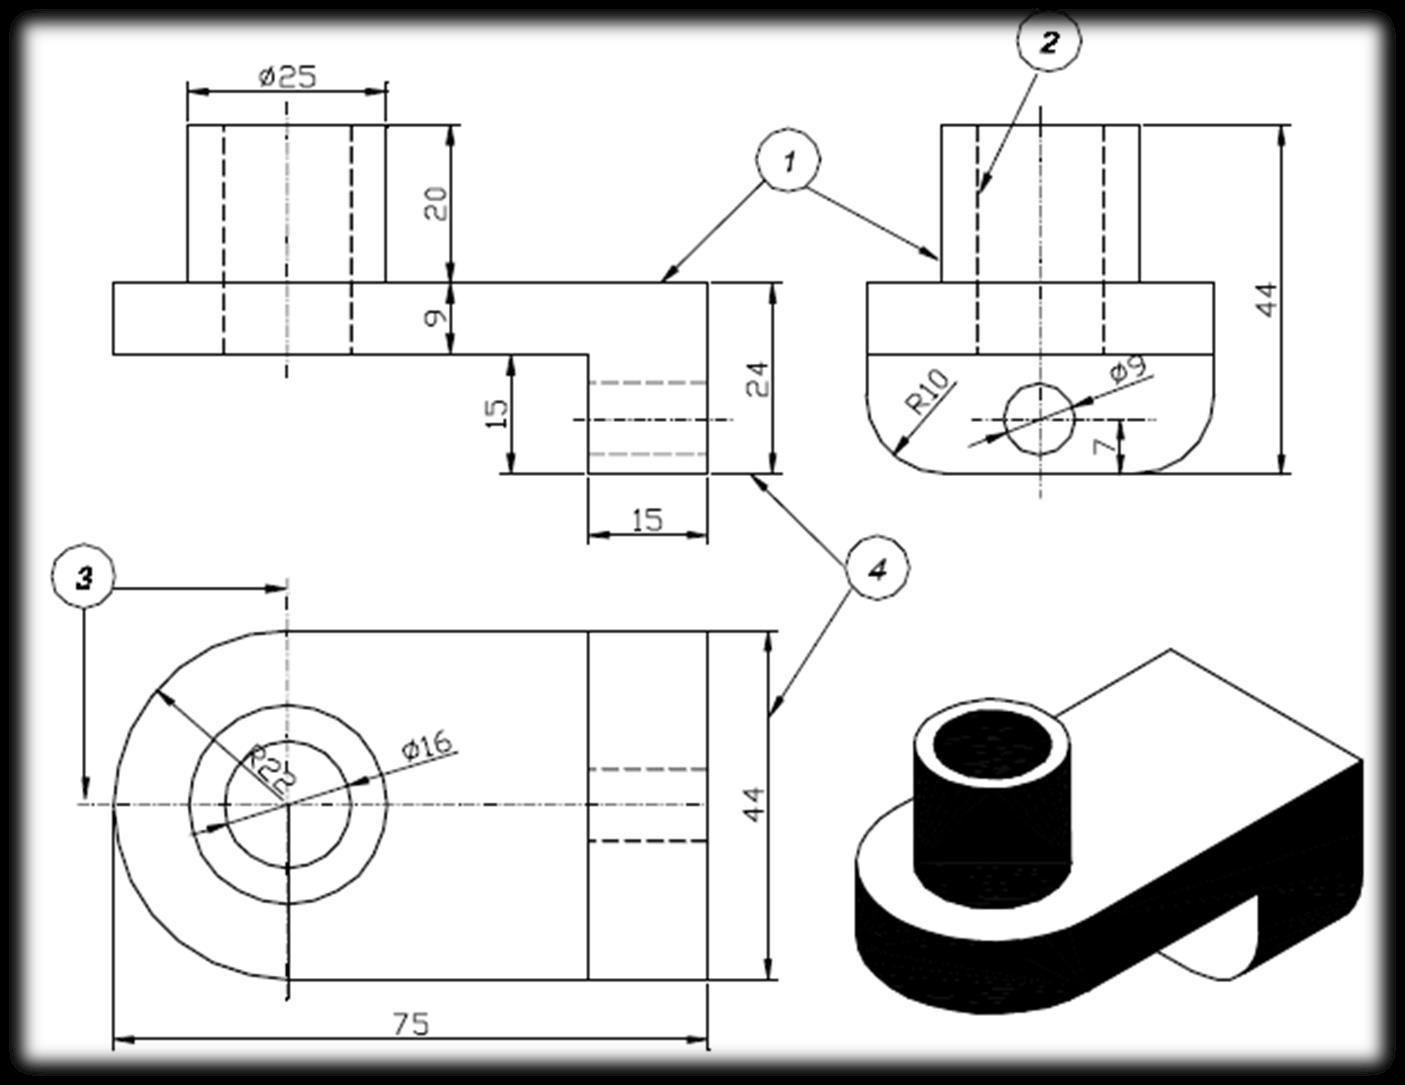
\includegraphics[height = 0.6\textheight]{img/desenho2.jpg}
                \caption{\cite{listade:online}}
            \end{figure}
        \end{column}

        \begin{column}{0.5\textwidth}
            \begin{figure}
                \centering
                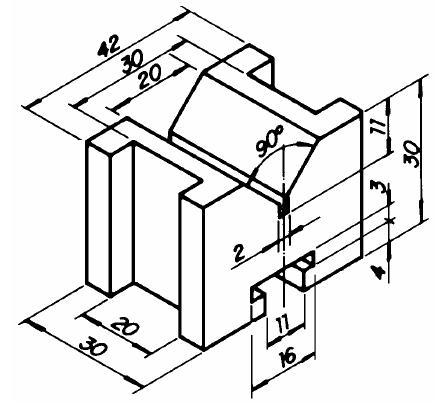
\includegraphics[height = 0.7\textheight]{img/desenho3.jpg}
                \caption{\cite{listade:online}}
            \end{figure}
        \end{column}
    \end{columns}
    
\end{frame}

\begin{frame}{Pratica 1}
    Realizar o desenho técnico da peça abaixo:
    \newline
    \begin{center}
        \begin{figure}
            \centering
            
\includegraphics[height = 0.5\textheight]{img/pratica1.png}
            \caption{\cite{Garrafa:online}}
        \end{figure}
    \end{center}
    
\end{frame}

\begin{frame}{Dever de casa}
    Realizar o desenho técnico da peça abaixo:
    \newline
    \begin{center}
        \begin{figure}
            \centering
            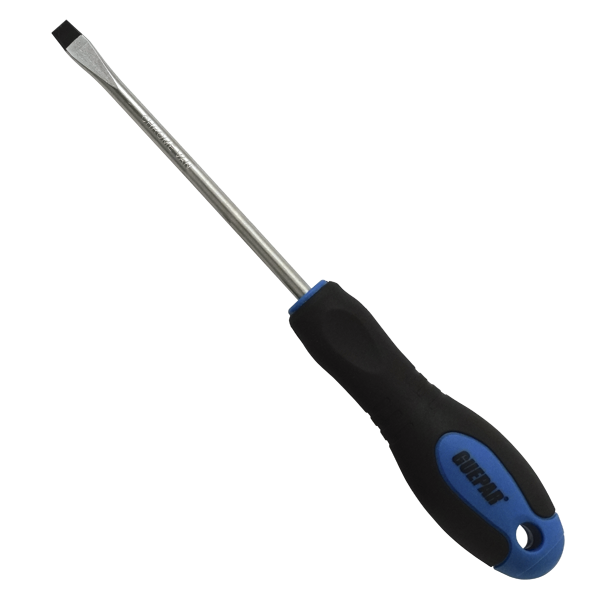
\includegraphics[height = 0.5\textheight]{img/dever1.png}
            \caption{\cite{Chavede:online}}
        \end{figure}
    \end{center}
    
\end{frame}

\section*{Esboço}



\begin{frame}[standout]
    \Huge\textsc{Thank You}
    
    \vfill
    
    \LARGE\textsc{Questions?}
\end{frame}
\begin{frame}[t, allowframebreaks]{References}
    \bibliographystyle{abntex2-alf}
    \bibliography{bibliography}
\end{frame}

\appendix

\begin{frame}{Backup slides go here}
    
\end{frame}

\end{document}
